% !TEX root = ../main.tex
% Daten

Dieses Kapitel erörtert die Struktur der Datensätze sowie die Methoden mit denen die Datensätze erstellt wurden.
Dabei wird im Detail auf zwei Datensätze eingegangen: der Wikipediadatensatz im XML-Format und eine spärlich besetzte Adjazenz-Matrix.
Der Abschnitt \ref{subchap:wikidump} erläutert, in welchem Format der Datensatz von Wikipedia vorliegt und welche Informationen aus diesem für die Visualisierung extrahiert werden können.
Im Abschnitt \ref{subchap:simmatrix} wird zum einen beschrieben, wie die dünn besetzte Matrix erstellt und zum anderen in welcher Struktur sie gespeichert wird.
Der nachfolgende Teil des Kapitels beschäftigt sich mit dem schematischen Aufbau der Datenbank.
Die Tabelle \ref{tab:dataset-size} zeigt die Größe der beiden Datensätze im Vergleich.

% und den notwendigen Schritten der S"auberung der Datens"atze zur erstelltung der Datenbank.

% Tabelle datensatz groesse
%NOTE: vllt groesse martin erste simMatrix
\begin{table}
\centering
% \begin{center}
\begin{tabular}{l r}
  \hline
  Datensatz & Größe \\
  \hline
  Wikipedia-Dump & 54 GB \\
  "Ahnlichkeitsmatrix & 642 GB \\
  \hline
\end{tabular}
% \end{center}
\caption{Größe der Datensätze in Gigabyte (GB)}
\label{tab:dataset-size}
\end{table}



 % =================================================
\section{Wikipedia XML Dump}
\label{subchap:wikidump}

% Datenstruktur wikipedia Korpus
%   groesse
%   namespaces
%   welche meta informationen werden extrahiert
%       titel, laenge, revid, wikiid, categories, 
% struktur Kategoriebaum
 
Der Wikipediadatensatz ist im XML-Format gespeichert und beinhaltet sämtliche Seiten der Wikipedia. 
Darunter fallen sowohl die jeweiligen Seiten auf der Portal-, Kategorien- und Artikelebene, als auch zusätzliche Seiten, wie das Impressum oder die Erklärungsseite über das Projekt der Wikipedia.
Dabei werden die unterschiedlichen Seiten in "`Wikipedia Namespaces"' eingeteilt [wns] \footnote{\url{https://en.wikipedia.org/wiki/Wikipedia:Namespace}}.
Die Tabelle \ref{tab:dataset-size} gibt Auskunft über die Größe eines solchen Wikipedia-Datensatzes.
Die vorliegende Arbeit beschränkt sich hierbei auf die für diese Analyse relevanten Artikelseiten aus dem [wns 0] sowie die Kategorienseiten aus dem [wns 14].
Aus diesen Seiten lassen sich alle Metainformationen extrahieren, die für eine visuelle Darstellung notwendig sind.
Der Tabelle \ref{tab:xml-overview} ist die genaue Anzahl der Artikelseiten und der Kategorienseiten zu entnehmen, welche im Wikipedia-Datensatz enhalten sind.

\begin{table}
\centering
\begin{tabular}{l r}
  \hline
  Art der Seite & Anzahl der Dokumente \\
  \hline
  sämtliche Wikipedia-Seiten & 16.527.332 \\
  Artikelseiten & 12.488.908 \\
  Kategorieseiten & 1.398.260 \\
  \hline
\end{tabular}
\caption{Verteilung der Artikel- und Kategorienseiten im Wikipedia-Datensatz, mit doppelten Seiten, Weiterleitungen und Vereindeutigungsseiten}
\label{tab:xml-overview}
\end{table}


Die im Anhang einsehbaren Auszüge \ref{xml-artikel} und \ref{xml-kategorie} stellen einen Ausschnitt aus dem Wikipedia-Dump für eine Artikel- und eine Kategorienseite dar.
Metainformationen wie der 'Titel', die 'Revisions-Id', die 'Wikipedia-Id' und der 'Namespace' können durch die definierten \emph{Elemente} des nach dem XML-Schema formatierten Wikipedia-Datensatzes mit geringem Aufwand extrahiert werden.
Diese Stellen sind in den Auszügen rot markiert, die blau markierten Stellen dagegen befinden sich innerhalb des \emph{Textelements}, also innerhalb des Fließtextes einer Wikipedia-Seite.
Um die Metainformationen über die Kategorienzugehörigkeit aus dem Fließtext extrahieren zu können, müssen reguläre Ausdrücke zur Extraktion geschrieben werden.

% Mit der Hilfe von regul"aren Ausdr"ucken k"onnen auch Metainformatione aus dem Flie"stext extrahiert werden, in diesem Fall die Kategorizugeh"origkeit.
% F"ur die Extraktion aller Metainformation aus dem Wikipediadatensatz wurde ein Programm geschrieben um die Daten in Datein zwischenspeichert um Sie dann mit dern Daten aus der "Ahnlihckeitsmatrix zusammen zuf"uhren.

Der Abschnitt \ref{subchap:date-pipeline} geht im Speziellen darauf ein, wie die Daten verarbeitet werden, damit die extrahierten Daten gemeinsam mit der Ähnlichkeitsmatrix in die Datenbank eingepflegt werden können.

\subsubsection{Filterung}
Die in Tabelle \ref{tab:dataset-size} dargestellten Zahlen beinhalten viele Seiten, die keiner Informationsgewinnung dienen.
Dazu gehören bespielsweise Seiten, welche als Weiterleitung auf andere Seiten fungieren. Diese Seiten gibt es sowohl auf der Artikelebene als auch auf der Kategorienebene.
Die zweite Art von Seite, welche inhaltslos sein kann, sind Artikelseiten, die zur Vereindeutigung dienen, wenn es mehrere Artikel zu einem Begriff mit verschiedenen Bedeutung gibt.
Im Anhang befinden sich Auszüge solcher Seiten.


 % =================================================
 

 % =================================================
\section{"Ahnlichkeitsmatrix}
\label{subchap:simmatrix}
% beide Arbeiten verwenden die Kosinusähnlichkeit als Ma"s für die Vergleiche
% Bezugname Arbeit von Potthast
%   Verwendetes "Ahnlichkeitesma"s 
%   Daten "uber die "Ahnlichkeiten (Anzahl)

% Bezugnahme zur Thesis von Tristan Licht
%   Verwendetes "Ahnlichkeitesma"s
%   "Ahnlichkeit von Paragraphen
%   Daten "uber die "Ahnlichkeiten (Anzahl)

% Inhalt der Matrix
% schematischer aufbau grafik
% Vergleich der zwei Datens"atze
 
% kurzer Absatz wie im Papert vta, was wurde wie berechnet
% kleine Tabelle??

In der Arbeit \emph{"`Visualizing Article Similarities in Wikipedia"'} \cite{riehmann2016visualizing} werden die Artikel der Wikipedia untereinander verglichen.
Dafür werden in einem ersten Schritt mit Hilfe der Stoppwort-Entfernung und dem Stemming für die jeweiligen Artikel Wortvektoren erstellt, welche nach dem TF-IDF-Modell gewichtet sind.
Gemeinsam bilden diese Vektoren eine Termdokumentenmatrix, mit welcher sich dann die Kosinusäahnlichkeiten berechnen lassen.
In einem nächsten Schritt werden die Wortvektoren in absteigender Rangordnung untereinander verglichen, wobei nur die Vergleiche gespeichert werden, die einen Ählichkeitswert über $0.1$ haben oder zu den $100.000$ höchsten Vergleichen mit einem Wert über $0.1$ gehören.
Damit die mögliche Anzahl an Berechnungen pro Artikel eingegrenzt werden kann und weiter sinkt, werden die Artikel mit einer Länge über 50 Wörtern mit allen Artikeln verglichen.
Dies bedeutet, dass längere Artikel mit kürzeren Artikeln verglichen werden, jedoch nicht kürzere untereinander.
Die enstandene Ähnlichkeitsmatrix beinhaltet im Vergleich 3.8 Millionen Artikel und hat eine Größe von 402 GB.
In der Grafik \ref{fig:simmatrix-1} wird der Aufbau schematisch dargestellt.
Das Ergebnis dieses Ansatzes ist jedoch, dass die einfache Kosinusähnlichkeit auf Artikelebene in ihrer Funktion als Vergleichsmaß als unzureichend einzustufen ist.

\begin{figure}
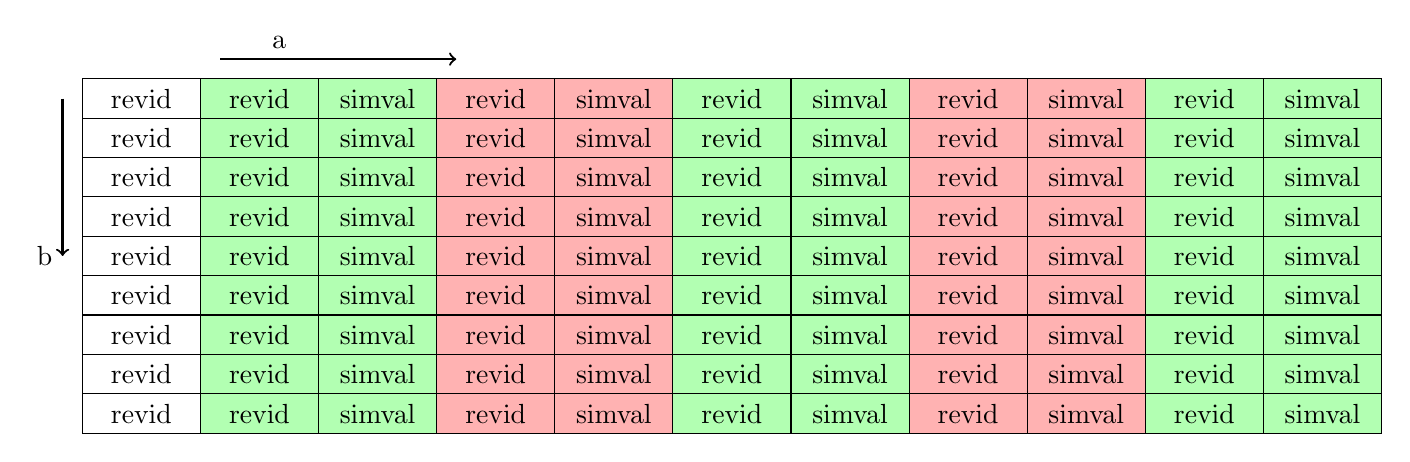
\begin{tikzpicture}[scale=1]
% first column
\draw[black, thick, ->] (2,5.5) -- (5,5.5) node[near start, above]{a};
\draw[black, thick, ->] (0,5) -- (0,3) node[left]{b};
% \draw (0,0) node {a: absteigende "Ahnlichkeitsewrte};
% \draw (6,0) node {b: absteigende Artikell"ange};
\foreach \y in {1,1.5,...,5}
{
    \draw (1,\y) +(-.75,-.25) rectangle ++(.75,.25);
    \draw (1,\y) node{revid};
}


\foreach \x in {2.5,4.0}
{
    \foreach \y in {1,1.5,...,5}
    \filldraw[fill=green!30] (\x,\y) +(-.75,-.25) rectangle ++(.75,.25);
    % \draw (\x,1) node{revid};
}
\foreach \x in {5.5,7.0}
{
    \foreach \y in {1,1.5,...,5}
    \filldraw[fill=red!30] (\x,\y) +(-.75,-.25) rectangle ++(.75,.25);
    % \draw (\x,1) node{revid};
}
\foreach \x in {8.5,10.0}
{
    \foreach \y in {1,1.5,...,5}
    \filldraw[fill=green!30] (\x,\y) +(-.75,-.25) rectangle ++(.75,.25);
    % \draw (\x,1) node{revid};
}
\foreach \x in {11.5,13.0}
{
    \foreach \y in {1,1.5,...,5}
    \filldraw[fill=red!30] (\x,\y) +(-.75,-.25) rectangle ++(.75,.25);
    % \draw (\x,1) node{revid};
}
\foreach \x in {14.5,16.0}
{
    \foreach \y in {1,1.5,...,5}
    \filldraw[fill=green!30] (\x,\y) +(-.75,-.25) rectangle ++(.75,.25);
    % \draw (\x,1) node{revid};
}
    
\foreach \y in {1,1.5,...,5} {
    \foreach \x in {2.5,5.5,...,16}
    {
        \draw (\x,\y) node{revid};
    }
    \foreach \x in {4.0,7.0,...,16}
    {
        \draw (\x,\y) node{simval};
    }
}
    
    % % revision
    % \foreach \x in {2.7,5.7,...,15}
    % {
    %     \filldraw[fill=green!30, thick] (\x,1.5) +(-.75,-.25) rectangle ++(.75,.25);
    %     \draw (\x,1.5) node{revid};
    % }
    % %simval
    % \foreach \x in {4.2,7.2,...,15}
    % {
    %     \filldraw[fill=red!30, thick] (\x,1.5) +(-.75,-.25) rectangle ++(.75,.25);
    %     \draw (\x,1.5) node{simval};
    % }
% }
\end{tikzpicture}
\caption{Schema der Ähnlichkeitsmatrix nach \cite{riehmann2016visualizing} \emph{a}: sortiert nach den absteigenden Ähnlichkeitswerten \emph{b}: sortiert nach der absteigenden Artikellänge}
\label{fig:simmatrix-1}
\end{figure}


% LICHT
% erwaehnen der selben daten und schritte wie in vta nur fuer licht thesis
Die Arbeit \emph{"`Eruierung von Methoden zur Exploration von Textwiederverwendung in großen Datenmengen am Beispiel der Wikipedia"'} \cite{licht:2017} baut auf den Ergebnissen von \cite{riehmann2016visualizing} auf, versucht im Gegensatz aber nicht auf Dokumentenebene, sondern auf Paragraphenebene die Vergleiche zu berechnen.
Dafür werden die Artikel anhand ihrer Überschriften in Paragraphen unterteilt.
Diese veränderte Schwerpunktsetzung hinsichtlich der Paragraphen soll die Suche nach Passagen durch die Textwiederverwendung verbessern.
Da die Vergleiche bei dieser Methode auf Paragraphenebene gezogen werden, vergrößert sich die Anzahl an möglichen Vergleichen signifikant, was wiederum eine neue Herausfordeung darstellt.

Die Artikel werden tokenisiert und von Stoppwörtern gesäubert.
Paragrpahen, die kürzer als 50 Wörter sind, werden mit dem vorherigem Paragraphen zusammengeführt. 
Artikel, welche eine Länge von 100 Wörtern unterschreiten, werden nicht für die Berechnung betrachtet.
Des Weiteren werden Artikel, die keinen Inhalt bieten, sondern lediglich zur Vereindeutigung dienen, ausgelassen.
Die Tabelle \ref{tab:simMatrix-overview} nach \cite{licht:2017} verdeutlicht die Reduzierung der Artikel durch die beschriebenen Schritte und die tatsächliche Anzahl an ermittelten Paragraphen, für welche die Ähnlichkeit berechnet wird.
Aus den daraus resultierenden Paragraphen berechnen sich eine Menge von $36,19$ Billionen Vergleichsoperationen.

\begin{table}
\centering
\begin{tabular}{l r}
  \hline
  & Anzahl \\
  \hline
  Seiten in wns 0 & 5.139.351 \\
  Seiten in wns 14 & 5.139.351 \\
  Artikel gefiltert durch Länge & 2.400.125 \\
  Artikel gefiltert durch Vereindeutigung & 118.468 \\
  Verbleibende Artikel & 2.620.758 \\
  Resultierende Paragraphen & 8.507.799 \\
  \hline
\end{tabular}
\caption{Übersicht der gefilterten Wikipedia-Artikel}
\label{tab:simMatrix-overview}
\end{table}

\begin{table}
\centering
\begin{tabular}{c r}
  \hline
  Kosinus\"ahnlichkeit & Anzahl der Dokumentenpaare \\
  \hline
  $[0.9,1.0]$ & $1.440.388$\\
  $[0.8,0.9)$ & $9.983.895$\\
  $[0.7,0.8)$ & $160.716.484$\\
  $[0.6,0.7)$ & $273.926.278$\\
  $[0.5,0.6)$ & $287.084.295$\\
  $[0.4,0.5)$ & $307.513.389$\\
  $[0.3,0.4)$ & $627.619.558$\\
  $[0.2,0.3)$ & $3.606.431.052$\\
  $[0.1,0.2)$ & $31.624.808.958$\\
  \hline
\end{tabular}
\caption{Verteilung der Ähnlichkeiten über die Artikel anhand ihrer ähnlichsten Paragraphen}
\label{tab:simMatrix-overview-sims}
\end{table}

Die Paragraphen, welche als TF-IDF gewichtet sind und als dünn besetzte Vektoren vorliegen, werden mit der Kosinusähnlichkeit untereinander verglichen.
Aus der Paragraphenmatrix wird zurück auf die Artikelebene abgebildet, in dem nur die Paragraphenpaare gespeichert werden, welche für ein Artikelpaar über die höchste Ähnlichkeit haben.
Anschlißend werden für die entsprechenden Paragraphen Representatnen in Form von TF-IDF gewichteten, dünn besetzten Wordvektoren erstellt.
Damit stehen die Paragraphen mit der höchsten Ähnlichkeit zueinenader stellvertretend für die Ähnlichkeit zwischen zwei Artikeln.
In \todotext{grafik ablauf s"auberung} ist ein schematischer Ablauf der beschriebenen Schritte zu sehen, während die Abbildung \todotext{grafik new simMatrix csv} den Aufbau einer Ähnlichkeitsmatrix nach \cite{licht:2017} zeigt.

Um die bestehende Pipeline zur Erstellung der Datenbank zu nutzen, sollte die Matrix nach \cite{licht:2017} dem Format der Matrix nach \cite{riehmann2016visualizing} entsprechen.

 % =================================================


 % =================================================
\section{Datenbankentwurf}
\label{subchap:database}
% erlaueterung der DAtenbankstruktur
% page table
% category table
% article table
Dieses Kapitel befasst sich mit dem Aufbau des Datenbankschemas sowie dem Gefüge aus \emph{FastDB} und \emph{WikiDB}.

\paragraph{FastDB und Datenbankschema}
Zur Speicherung der Daten wird eine In-Memory-Datenbank nach \cite{fastdb} genutzt, auf diese Art wird der Zugriff auf die Daten beschleuningt.
Die \emph{FastDB} nach \cite{fastdb} ist eine Objekt-Relationale-Datenbank \footnote{\url{https://en.wikipedia.org/wiki/Object-relational_database}}.
Die Datenbank wird durch sogenannte Klassen modelliert: Die jeweiligen Klassen stellen dabei die einzelnen Tabellen dar und die Instanzen der Klassen entsprechen den Zeilen einer Tabelle.
Die Variablen einer Klasse sind die Spalten der Tabellen dieser Datenbank.
In der Abbildung \ref{fig:uml-database} wird der Aufbau der Datenbank verdeutlicht.
In der Klasse \emph{page} sind die Eigenschaften vereint, welche für die Seiten mit den jeweiligen Wikipedia-Namensräumen zutreffen, wie der Titel, die Revisions-Id oder eine Liste von Kategorien, in welchen die Seite eingetragen ist.
Die Seiten Klassen \emph{article} und \emph{category} stellen Spezialisierungen der Klasse \emph{page} dar.
Ein \emph{article} besitzt zusätzlich zu den Eigenschaften einer \emph{page} eine bestimmte Anzahl an Wörtern, genauso wie eine Liste von vergleichbaren Artikeln.
Diese Liste der vergleichbaren Artikel macht den Großteil der Datenbank aus, dabei entsprechen die Listen mit den Vergleichspaaren den Zeilen aus der Ähnlichkeitsmatrix.
Die Klasse der \emph{category} hingegen verfügt über keine Artikelvergleiche, dafür aber über eine Liste mit weiteren Kategorien, welchen sie angehört.
Die Datenbank enthält zudem Informationen darüber, welche Artikel oder Kategorien ebenfalls in anderen Kategorien erwähnt werden.
Die Verknüpfungen werden dabei bidirektional eingetragen, somit lässt sich aus einer Kategorie ablesen, welche Artikel oder Kategorien in derjenigen eingetragen sind.
Dieser Schritt ermöglicht schließlich die Konstruktion eines Kategoriengraphen aus dem Wikipedia-Datensatz und ist zudem die Grundlage für die später folgende visuelle Darstellung der Kategorien in Form eines Baumes.
Auf diese Weise übernimmt die Datenbank nicht nur die Aufgabe die Daten zu speichern und zugänglich zu machen, sondern erweitert die Informationen aus dem Wikipedia-Datensatz um die Zugehörigkeit von Artikeln und Kategorien zu weiteren Kategorien.
Die Datenbank bildet somit Teile aus der Wikipedia, als auch Teile aus der Ähnlichkeitsmatrix ab und ermöglicht den Zugriff auf die extrahierten Informationen aus den Daten.

\paragraph{WikiDB}
Die \emph{WikiDB} ist eine Hülle, welche um die Datenbank herum konstruiert ist.
Sie erleichtert die Interaktion mit der Datenbank, indem sie die Interaktion auf die Abstraktionsebene von Artikeln, Kategorien und Vergleichen hebt.
Dabei übernimmt die \emph{WikiDB} auch Teile der Konstruktion der Datenbank und ermöglicht eine Suche nach Artikeln oder Kategorien, sie ist als Schnittstelle zwischen Daten und Applikation zu verstehen.
Im Anhang ist ein Auschnitt aus den Funktionalität der \emph{WikiDB} dargestellt. \todotext{refeinfügen}


\tikzumlset{fill class=white}
\begin{figure}
\begin{tikzpicture}
\centering
\umlclass[x=0, y=0]{page}{
+index : int4   \\
+revid : int4   \\
+title : char const*\\
+parents : dbArray<dbReference<Category>>\\
} {
+info() : std::string const \\
+getParents() : std::vector<Category> const \\
}

\umlclass[x=-5, y=-6]{article}{
+words : int4\\
+comparisons : dbArray<int64\_t> \\
}{
+info() : std::string const \\
+getComparisons() : std::vector<SimPair> const \\
}

\umlclass[x=5, y=-6]{category}{
+children : dbArray<dbReference<Page> >\\
}{
+info() : std::string const \\
+getChildren() : std::vector<uint32\_t> const\\
}
\umlVHVinherit{category}{page}
\umlVHVinherit{article}{page}
\end{tikzpicture}
\caption{UML Diagramm der Klassen für die objekt-relationale Datenbank}
\label{fig:uml-database}
\end{figure}

% =================================================
 
 % =================================================
\section{Ablauf der Datenaufbereitung}
\label{subchap:date-pipeline}
% Aufbereitung Rohdaten: Säuberung, Formatierung
    % regex: 
    % from csv to tsv
    % new wikiformat?
% Erstellung der Datenbank
\todotext{Bild Ablauf Entstehung Matrix (Notizen Skizze)}

Die vorangegangenen Kapitel setzen sich mit der Beschaffenheit der in dieser Arbeit untersuchten Datensätze auseinander. Dieses Kapitel behandelt die weitere Datenverarbeitung; wie sollten die Daten verarbeitet werden, damit sie in die Datenbank eingepflegt werden können? Welche Maßnahmen sind erforderlich, um die Daten vor möglichen Fehlerquellen zu schützen?
Dabei wird darauf eingegangen, welche Probleme auftreten können, wenn erstens die Datensätze von Menschen erzeugt werden und nicht mit absoluter Gewissheit gewährleistet werden kann, dass die Daten einem festgelegten Regelwerk entsprechen. Zweitens wird gezeigt, in welcher Art die Daten fehlerhaft oder nicht vollständig sein können und wie damit umgegangen wird.
Abschließend wird exemplarisch dargestellt, wie aus den einzelnen Datensätzen eine Datenbank konstruiert wird.

\subsubsection*{Ähnlichkeitsmatrix}
In der Ähnlichkeitsmatrix von \cite{riehmann2016visualizing} wurde zur Identifizierung der einzelnen Artikel ihre jeweilige Revisionsnummer genutzt.
Mit dieser Nummer lässt sich die exakte Version des Artikels rekonstruieren, mit dem die Berechnung für den Vergleich durchgeführt wurde.
In der Arbeit von \cite{licht:2017} hingegen wurde auf die Nutzung der Revisionsnummer verzichtet. Stattdessen wird die Wikipeida-Identifikationsnummer, im Folgenden \emph{wikiid}, genutzt.
Aus der Rekonstruier- und Nachvollziehbarkeit wird dieser Unterschied in den Datensätzen angepasst und auf das Format von \cite{riehmann2016visualizing} übertragen. Somit besteht die Möglichkeit, neben dem gespeicherten Artikel im Wikipedia-Datensatz, auch mit einer API-Anfrage die exakte Version des Artikels zu erhalten.
Auf diese Weise ist der gespeicherte Datensatz nicht die einzige Quelle für die Rekonstruktion der Datenbank, sollte der Datensatz nicht mehr verfügbar sein.
Damit eine \emph{wikiid} in eine Revisionsnummer aufgelöst werden kann, ist es nötig, beim Durchlaufen des Wikipedia-Datensatzes zur Extraktion der Metainformationen die Abbildung der \emph{wikiid} auf die Revisionsnummer hin zu speichern.
Zur Vereinfachung wurde im Anschluss die gesamte Ähnlichkeitsmatrix von \emph{wikiids} auf Revisionsnummern hin verändert.

\subsubsection*{Wikipedia-Datensatz}
Das Format des Wikipedia-Datensatzes wird durch ein XML-Schema \footnote{\url{https://www.mediawiki.org/xml/export-0.10.xsd}} definiert.
Wird das XML-Schema erneuert, muss diese Änderung auch in dem Werkzeug zur Extraktion der Metainformationen berücksichtigt werden.
% Diese Anpassung des Programms an die Version des XML-Schemas ist keine Herausforderung.
Der Wikipedia-Datensatz benutzt dabei nicht nur XML als Auszeichnungssprache, sondern auch eine eigene Auszeichnungssprache, die \emph{Wiki Markup Language} \footnote{\url{https://en.wikipedia.org/wiki/Help:Wiki\_markup}}. 
Diese Auszeichnungssprache wird innerhalb der Textelemente der XML-Datei genutzt und ermöglicht eine Formatierung des geschriebenen Textes.
Hinzu kommt die Möglichkeit, mit Hilfe der \emph{Wiki Markup Language} auch interne Verknüpfungen auf andere Wikipedia-Seiten herzustellen.
Extrahiert werden alle Seiten, die im Wikipedia-Namensraum 0 oder 14 liegen, also Artikelseiten oder Kategorieseiten entsprechen.
Relevant für diese Arbeit ist, dass Artikel- oder Kategorienseiten, welche entweder eine Weiterleitung \footnote{\url{https://en.wikipedia.org/wiki/Template:Disambiguation}} oder eine Vereindeutigung \footnote{\url{https://en.wikipedia.org/wiki/Template:Redirect}} darstellen, nicht mit extrahiert werden.
Für diesen Fall wurden reguläre Ausdrücke geschrieben, die Seiten dieser Art filtern sollen. Zudem wurden für die Extraktion von Kategoriezugehörigkeiten reguläre Ausdrücke entwickelt.
Die Extraktion der Kategorien aus den Wikipedia-Seiten ist ein Kernelement der Datenextraktion und nötig um im weiteren Prozess der Visualisierung ihre hierarchische Struktur darzustellen.
Zu beachten ist, dass die regulären Ausdrücke angepasst werden müssen, sobald sich die \emph{Wiki Markup Language} ändert.

\paragraph{Verarbeitung}
Zwei Werkzeuge wurden weiterentwickelt, um diesen neuen Anforderungen zu entsprechen, das \emph{wikitool} und \emph{createdb}.
Die Grafik \todotext{3.4} veranschaulicht die Datenverarbeitung durch die Werkzeuge \emph{wikitool} und \emph{createdb}.

Als Datensatz zur Eingabe wird der Wikipedia-Datensatz mit verschiedenen Parametern aufgerufen.
Zunächst (\emph{extract}) werden aus dem Datensatz die Metainformationen zu den entsprechenden Kategorien extrahiert und in einer TSV-Datei gespeichert.
In einem nächsten Schritt werden die Metainformationen zu den Artikeln zwischengespeichert und im dritten Schritt (\emph{clean}) mit dem Inhalt der Ähnlichkeitsmatrix abgeglichen, damit nur Artikel aus dem Wikipedia-Datensatz in die Datenbank eingetragen werden, welche auch in der ersten Spalte der Ähnlichkeitsmatrix stehen.
Der zweite Schritt (sample) ist dabei optional und ermöglicht durch ein Stichprobenverfahren den Datensatz zu verkleinern.
Die Stichprobe kann dabei zufällig oder geschichtet sein. 
Mit dieser Methode lassen sich kleinere Datesätze erstellen, die als Musterexemplar dienen können.
\\
Das Werkzeug \emph{createdb} hingegen konstruiert in drei aufeinander folgenden Schritten die Datenbank.
Dabei werden erst alle Seiten im Schritt (\emph{pages}) mit ihrem Titel, ihrer Identifikationsnummer und Artikel mit ihrer Anzahl an Wörtern eingefügt.
Der Schritt (\emph{parents}) ergänzt die bereits eingetragenen Seiten um die Liste von Kategorien, in denen die Seiten eingeordnet werden.
Zuletzt werden die Artikelseiten im Schritt (\emph{comparisons}) um die Liste der verglichenen Seiten und ihren Ähnlichkeiten ergänzt.

Die erzeugte Datenbank kann in den gemeinsam genutzten Speicher kopiert werden und dient der Visualisierung.


\begin{figure}
    \centering
    \begin{tikzpicture}[scale=1.5, page/.style={rectangle, draw, fill=white, rounded corners, minimum size = 1cm}]
    %boxes
        \node[page] (simM)      at(-3,5)    {"Ahnlichkeitsmatrix};
        \node[page] (wikidump)  at(-2.8,3)    {Wikipediadump};
        \node[page, align=center] (wikitool)    at(-0.5, 4)   {wikitool/\\createdb};
        \node[page] (wikidb)    at(1.3, 4)   {wikidb};
        \node[page, align=center] (mapper)    at (3.5,4)    {Objekt-Relation-\\Abbildung};
        \node[page, align=center] (app)       at (6,4)    {OpenGl-\\Applikation};
        
        \draw[decoration={brace, mirror}, decorate] (-3,2.5) node[below]{testing} -- (0,2.5);
    
    % lines
        \draw[-{triangle 60}] (simM.east) -- (wikitool.west);
        \draw[-{triangle 60}] (wikidump.east) -- (wikitool.west);
        \draw[-{triangle 60}] (wikitool.east) -- (wikidb.west);
        \draw[-{triangle 60}] (wikidb.east) -- (mapper.west);
        \draw[-{triangle 60}] (mapper.east) -- (app.west);
    
    \end{tikzpicture}
    \caption{Ablauf der einzelnen Schritte, von den Rohdaten zur Konstruktion der Datenbank}
    \label{fig:ablauf-daten}
\end{figure}


\begin{figure}
    \centering
    \begin{tikzpicture}
        \filldraw[color=black, fill=white, thick] (-5,4.5)       rectangle (-4,3);
        \filldraw[color=black, fill=white, thick] (-5.1,4.6)   rectangle (-4.1,3.1);
        \filldraw[color=black, fill=white, thick] (-5.2,4.7)   rectangle (-4.2,3.2);
        \draw[decoration={brace, mirror}, decorate] (-6,2.5) node at(-5,1.5){Wikipedia XML Datei} -- (-3.5,2.5);
        
        \draw[-{triangle 60}] (-3,4) -- (-2.5,4);
        \node[draw, rectangle, align=left] at (-1, 4) {1. extract\\(2. sample)\\3. clean};
        \draw[decoration={brace, mirror}, decorate] (-2.5,2.5) node at(-1,1.6){wikitool} -- (0.5,2.5);
        
        \draw[-{triangle 60}] (0.5,4) -- (1,4);
        \filldraw[color=black, fill=white, thick] (1.7,4.5)   rectangle   (2.7,3);
        \filldraw[color=black, fill=white, thick] (1.6,4.6) rectangle   (2.6,3.1);
        \filldraw[color=black, fill=white, thick] (1.5,4.7)   rectangle (2.5,3.2);
        \draw[decoration={brace, mirror}, decorate] (1.5,2.5) node at(2,1.6){TSV Dateien} -- (3.0,2.5);
        
        \draw[-{triangle 60}] (3,4) -- (3.5,4);
        \node[draw, rectangle, align=left] at (5.5, 4) {1. pages\\2. parents\\3. comparisons};
        \draw[decoration={brace, mirror}, decorate] (4,2.5) node at(5.5,1.6){createdb} -- (7,2.5);
        
        \draw[-{triangle 60}] (7.5,4) -- (8,4);
        \node[cylinder, draw, rotate=90, minimum height=1cm, minimum width=1.5cm] at (9, 4){};
        \draw[decoration={brace, mirror}, decorate] (8,2.5) node at(9,1.6){Datenbank} -- (10,2.5);
        
    \end{tikzpicture}
    \caption{Caption}
    \label{fig:my_label}
\end{figure}

% =================================================